\documentclass[11pt]{book}
\usepackage{hyperref}
\usepackage{amsfonts}
\usepackage{amssymb}
\usepackage{amsmath}
\usepackage[utf8]{inputenc}
\usepackage[T1]{fontenc}
\usepackage{float}
\usepackage{fixltx2e}
\usepackage[italian]{babel}
\usepackage{graphicx}

\newenvironment{sistema}%
{\left\lbrace\begin{array}{@{}l@{}}}%
{\end{array}\right.}


\title{Appunti di Ricerca Operativa}
\author{Fabio Viola}
\date{}

\setcounter{chapter}{5}

\begin{document}

\chapter{Programmazione Lineare Intera}

\scriptsize
{\bf Slide}:
\href{http://www.or.deis.unibo.it/staff_pages/martello/Chapter6.zip}{Integer
Linear Programming}
\normalsize
\vspace{20pt}

In molti problemi di interesse pratico le variabili non possono
assumere valori frazionali, basti pensare ad esempio al numero di
veicoli da impiegare su una data tratta. Ecco da dove nasce dunque la
necessit\`a di formulare problemi di {\bf programmazione lineare
  intera}. Tali problemi si presentano in una forma molto simile a
quella dei problemi di LP visti finora, con l'unica aggiunta del
vincolo di interezza:

\vspace{11pt}
\begin{center}
  \begin{tabular}{l}
    $\min c'x$\\
    $\phantom{min}Ax = b$\\
    $\phantom{min}x \geq 0$\\
    $\phantom{min}x intero$\\
  \end{tabular}
\end{center}
\vspace{11pt}

Se rimuovessimo il vincolo di interezza otterremmo il cosiddetto {\bf
  rilassamento continuo} del problema. Risolvendo tale problema
ricaveremmo una soluzione $z(LP)$ che \`e legata a $z(ILP)$ dalla
seguente {\bf propriet\`a}: $z(LP) \leq z(ILP)$ (trattandosi di
problemi di minimizzazione).

\vspace{11pt} $\square$ {\bf Dimostrazione}: cerchiamo un minimo in un
insieme pi\`u grande.  $\blacksquare$
\vspace{11pt}

$z(LP)$ \`e detto {\bf lower bound} di $z(ILP)$. Se $z(LP)$
corrisponde ad un punto intero $x \in \mathcal{R}^n$ , allora $x$ \`e
{\bf ottimo} per il problema di programmazione lineare intera.

Geometricamente possiamo dire che studiare un problema di ILP consiste
nell'analizzare soltanto i punti con coordinate intere del
poliedro. La soluzione ottima \`e uno fra questi punti. In prima
analisi potremmo pensare di risolvere un problema di programmazione
lineare intera semplicemente risolvendo il suo rilassamento continuo
ed arrotondando il risultato al pi\`u vicino intero.

Un primo algoritmo per fare ci\`o \`e:

\small
\vspace{11pt} 
\begin{center}
\begin{tabular}{||l||}
\hline\hline
{\bf procedure LIGABUE}:\\
{\bf begin}\\
\phantom{aaa}find the optimal solution $x$ to the continuous relaxation LP of the ILP;\\
\phantom{aaa}{\bf if} LP is impossible {\bf then} ILP is impossible
{\em (sicuramente vero)}\\
\phantom{aaa}{\bf else}\\
\phantom{aaaaaa}{\bf if} LP is unbounded {\bf then} ILP is unbounded
        {\em ('normalmente' vero)}\\
\phantom{aaaaaa}{\bf else}\\
\phantom{aaaaaaaaa}{\bf if} {\em x} is integer then $x^* := x$
{\em (sicuramente vero)}\\
\phantom{aaaaaaaaa}{\bf else} round each fractional $x_j$ to its closest integer\\
{\bf end}.\\
\hline\hline
\end{tabular}
\end{center}
\vspace{11pt} 
\normalsize

Questo metodo tuttavia non funziona, come possiamo vedere dalla figura
\ref{ligabue}. Nel primo grafico vediamo che la pi\`u vicina soluzione
intera potrebbe ancora essere inammissibile quindi servirebbero pi\`u
iterazioni, nel secondo invece vediamo che l'intero e la soluione
continua possono essere veramente lontani.

\begin{figure}[h!]
  \centering
  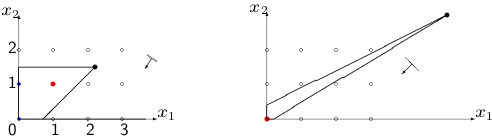
\includegraphics[width=0.8\textwidth]{images/ligabue.png}
  \caption{Arrotondamento della soluzione}
  \label{ligabue}
\end{figure}

Ora introduciamo una nozione che poi riprenderemo pi\`u
avanti. Parliamo dell'{\bf unimodularit\`a}. Una matrice intera
quadrata {\em B} \`e {\bf unimdulare} se $det(B) = \pm  1$.

Una  matrice intera rettangolare $m \times n$ {\em A} \`e {\bf
  totalmente unimodulare} se ogni sotto matrice quadrata non singolare
di {\em A} \`e unimodulare.

{\bf Propriet\`a}: se {\em A} \`e {\em TUM} (totalmente unimodulare),
allora i vertici del problema $\{x : Ax=b, x \geq 0 \}$ (che come
vediamo \`e in forma standard) sono interi per ogni {\em b} intero.

\vspace{11pt}
$\square$ {\bf Dimostrazione}: prendiamo la matrice {\em B}
corrispondente alla base di {\em A}. La soluzione di base \`e $x =
B^{-1}b = \frac{B^a}{det(B)}\cdot b$ dove $B^a$ \`e la {\bf matrice
  aggiunta} di {\em B}. Se {\em A} \`e TUM, {\em B} \`e {\em UM},
dunque {\em x} \`e intero. $\blacksquare$
\vspace{11pt}

{\bf Propriet\`a}: se {\em A} \`e {\em TUM}, allora i vertici di $\{ x :
Ax \leq b, x \geq 0 \}$ (problema in forma canonica) sono interi per
ogni {\em b} intero.

\vspace{11pt}
$\square$ {\bf Dimostrazione}: \`e sufficiente mostrare che se {\em A}
\`e {\em TUM} allora $(A|I)$ \`e {\em TUM}. Prendiamo allora {\em C},
una sottomatrice non singolare quadrata di $(A|I)$. Permutiamo le
righe di {\em C} in modo da avere $\tilde{C}$.

Abbiamo $det(\tilde(C)) = det(B)$ quindi $det(C) = \pm det(\tilde{C})
= \pm 1$. $\blacksquare$
\vspace{11pt}

Quindi se {\em A} \`e {\em TUM} l'algoritmo del simplesso riesce a
risolvere i problemi di programmazione lineare intera. Peccato che non
sia facile determinare quando una matrice \`e {\em TUM}.

Lasciamo ora da parte quest'argomento per concentrarci sui metodi
generali di risoluzione dei problemi ILP. In generale abbiamo due
famiglie di metodi risolutivi: {\bf piani di taglio} e {\bf branch and
  bound}.

\section{Piani di taglio}

Vediamo come si procede con un generico algoritmo di taglio.

Prendiamo il caso generale, quello in cui il rilassamento continuo \`e
{\bf limitato} e {\bf non vuoto}:

\begin{enumerate}
\item risolviamo il rilassamento lineare e troviamo la soluzione
  ottima $x^*$;
\item se $x^*$ \`e intero allora il problema \`e {\bf risolto},
  altrimenti:
\item aggiungiamo al problema {\em ILP} un vincolo lineare che
  soprannominiamo {\bf taglio} che:

  \begin{enumerate}
  \item elimina una parte della soluzione ammissibile contenente $x^*$;
  \item ma non elimini alcun punto intero della regione;
  \end{enumerate}

\item risolviamo il rilssamento lineare del nuovo problema e, trovato
  il nuovo $x^*$ ritorniamo al punto 2.

\end{enumerate}

\begin{figure}[h!]
  \centering
  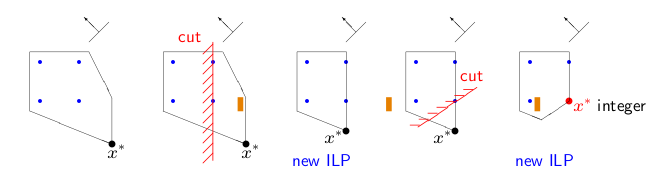
\includegraphics[width=0.9\textwidth]{images/esempiotagli.png}
  \caption{Un esempio di algoritmo di taglio}
  \label{esempiotagli}
\end{figure}

\subsection{Tagli di Gomory}

Vediamo nello specifico l'algoritmo dei {\bf tagli di
  Gomory}. Iniziamo definendo il concetto di {\bf parte
  intera}. $\forall y \in \mathcal{R}^1$, la parte intera di $y$ \`e
$\lfloor y \rfloor = \max q : q \leq y$ (con $q$ intero). $\lfloor y
\rfloor$ \`e dunque il pi\`u grande intero minore di $y$. Ad esempio
$\lfloor 7,95 \rfloor = 7$, $\lfloor -4,85 \rfloor = -5$.

Consideriamo ora il tableau finale del rilassamento continuo di un
problema e chiamiamolo {\em Y}. Al suo interno avremo una base ottima
$\mathcal{B}$. Nel tableau abbiamo la variabile $-z$ che possiamo
prendere come ulteriore variabile in base e chiamarla dunque
$x_{\beta(0)}$.

Scegliamo una qualunque riga $i \in 0 \dots m$. Se moltiplico i
coefficienti contenuti in quella riga (nella parte di tableau
afferente ad {\em A}) per {\em x} otterr\`o (ovviamente) il termine
noto {\em b} di quella riga:

\begin{center}
$y_{i0} = x_{\beta(i)} + \sum\limits_{A_j \not\in \mathcal{B}} y_{ij}x_j = y_{i0}$  
\end{center}

Per qualunque {\em i} ci\`o dev'essere verificato e $x$ dev'essere
maggiore o uguale a zero. 

Prendendo la parte intera, tale relazione diventa:

\begin{center}
$y_{i0} = x_{\beta(i)} + \sum\limits_{A_j \not\in \mathcal{B}} \lfloor y_{ij}
  \rfloor x_j = \lfloor y_{i0} \rfloor$
\end{center}

e facendo la differenza fra le due relazioni appena introdotte
otteniamo:

\begin{center}
  $\sum\limits_{A_j \not\in \mathcal{B}} (y_{ij} - \lfloor y_{ij} \rfloor) x_j
  \geq (y_{i0} - \lfloor y_{i0} \rfloor)$
\end{center}

Possiamo definire {\bf parte frazionaria} di $y_{ij}$ l'elemento
$f_{ij} = y_{ij} - \lfloor y_{ij} \rfloor$ con $0 \leq f_{ij} <
1$. Sulla base di questo nuovo concetto possiamo dunque riscrivere la
precedente formula come:

\begin{center}
$\sum\limits_{A_j \not\in \mathcal{B}} f_{ij}x_j \geq f_{i0}$  
\end{center}

Questo che abbiamo appena introdotto \`e detto {\bf taglio di Gomory}
della riga {\em i}.

Moltiplicando tale taglio per $-1$ ed aggiungendo una {\em variabile
  di slack} (necessaria per far si che il problema rimanga in forma
standard) otteniamo la nuova riga da inserire nel tableau:

\begin{center}
$-\sum\limits_{A_j \not\in \mathcal{B}} f_{ij}x_j + s = - f_{i0}$  
\end{center}

{\bf Teorema:} Aggiungendo la riga appena vista al tableau:

\begin{enumerate}
\item nessun punto intero ammissibile viene eliminato;
\item il tableau risultante contiene una base che sar\`a:

  \begin{enumerate}
  \item inammissibile per il primale, se $y_{i0}$ non \`e intero;
  \item ammissibile per il duale.
  \end{enumerate}

\end{enumerate}

\vspace{11pt}
$\square$ {\bf Dimostrazione}: dimostriamo il punto 1. Il taglio \`e
stato ottenuto imponendo semplicemente il vincolo di integralit\`a al
problema di LP;

Per quanto riguarda il punto 2.1, diciamo che $s$ \`e una nuova
variabile in base. Aggungendo $s$ in base otteniamo una base pi\`u
grande la cui soluzione include $s = -f_{i0} \leq 0$, dunque \`e
inammissibile per il primale visto che \`e minore di 0 se $y_{i0}$ non
\`e intero.

Per il punto 2.2, nella riga 0, la colonna corrispondente a {\em s} ha
uno 0, quindi la soluzione rimane ammissibile per il duale.

$\blacksquare$
\vspace{11pt}

\`E dunque conveniente continuare ad utilizzare l'algoritmo del
simplesso, anche se non risolve direttamente i problemi di ILP. La
riga {\em i} che selezioniamo per applicare il taglio \`e detta {\bf
  riga generatrice}.

Vediamo ora come si pu\`o riassumere l'algoritmo in pseudocodice:

\small
\vspace{11pt}
\begin{center}
\begin{tabular}{||l||}
\hline\hline
{\bf procedure GOMORY:}\\
{\bf begin}\\
\phantom{aa}remove the integrality constraints from the ILP thus obtaining an LP;\\
\phantom{aa}{\bf call TWO PHASE} for LP, and let Y be the final tableau;\\
\phantom{aa}{\bf if} infeasible = false {\bf and} unbounded = false {\bf then}\\
\phantom{aaaa}{\bf begin}\\
\phantom{aaaaaa}feasible := true; k := 0 {\em (commento: azzero il contatore)};\\
\phantom{aaaaaa}{\bf while} $\exists$ fractional $y_{i0}$ {\bf and} feasible = true {\bf do}\\
\phantom{aaaaaaaa}{\bf begin}\\
\phantom{aaaaaaaaaa}select an i : $y_{i0}$ is fractional, and set k := k + 1;\\
\phantom{aaaaaaaaaa}add the equation $- \sum\limits_{A_j \not \in \mathcal{B}} f_{ij} x_{j} + s_k = -f_{i0}$ to the tableau;\\
\phantom{aaaaaaaaaa}{\bf call DUAL SIMPLEX};\\
\phantom{aaaaaaaaaa}{\bf if} infeasible = true {\bf then}\\
\phantom{aaaaaaaaaaaa}feasible := false {\em (commento: duale
  illimitato, ILP impossibile)}\\
\phantom{aaaaaaaa}{\bf end}\\
\phantom{aaaa}{\bf end}\\
{\bf end.}\\
\hline\hline
\end{tabular}
\end{center}
\vspace{11pt}
\normalsize

Anche in questo caso la convergenza dell'algoritmo dipende dalla
degenerazione: se non ci sono basi degeneri, allora ogni volta
generiamo basi diverse e quindi l'algoritmo sicuramente converge,
altrimenti bisogna far qualcosa. Nello specifico noi agiremo con un
procedimento simile alla {\em regola di Bland} scegliendo la prima
riga frazionaria.

\vspace{11pt}
$\blacktriangleright$ {\bf Esempio}: consideriamo il seguente
problema:

\vspace{11pt}
\begin{center}
  \begin{tabular}{l}
    $\min -x_2$\\
    $\phantom{min}3x_1 + 2x_2 \leq 6$\\
    $\phantom{min}-3x_1 + 2x_2 \leq 0$\\
    $\phantom{min}x_1, x_2 \geq 0$, intere\\
  \end{tabular}
\end{center}
\vspace{11pt}

Tale problema non \`e espresso in forma standard perci\`o lo
riconduciamo subito:

\vspace{11pt}
\begin{center}
  \begin{tabular}{l}
    $\min -x_2$\\
    $\phantom{min}3x_1 + 2x_2 + x_3 = 6$\\
    $\phantom{min}-3x_1 + 2x_2 + x_4 0$\\
    $\phantom{min}x_1, x_2, x_3, x_4 \geq 0$, intere\\
  \end{tabular}
\end{center}
\vspace{11pt}

Come possiamo notare, abbiamo gi\`a una base... Costruiamo il primo
tableau inserendo $b=6$ e $A=\{3, 2, 1, 0 \}$ nella riga 1 e $b=0$, $A
= \{ -3, 2, 0, 1\}$ nella riga 2. A questo punto completiamo la riga 0
inserendo $-z = -(-x_2) = (x_2) = 0$ (dal momento che $x_2$ \`e una
variabile fuori base e quindi il suo valore \`e 0). I costi delle
variabili in base sono chiaramente 0. Ci restano da riempire i costi
delle altre due variabili fuori base tenendo presente la formula:

\begin{center}
$\bar{c}_j = c_j - \sum\limits_{i=1}^m y_{ij}c_{\beta(i)}$
\end{center}

Per la colonna $j = 1$ il costo \`e: $\bar{c}_1 = c_1 - ( y_{11} \cdot
c_{\beta(1)} + y_{21} \cdot c_{\beta(2)}) = 0 - (3 \cdot 0 - 3 \cdot
0) = 0$. Per la colonna $j = 2$ il costo \`e: $-1 - (2 \cdot 0 + 2
\cdot 0) = -1$.

Quindi il tableau risultante \`e quello di figura \ref{cap6tab1}.

\begin{figure}[h!]
  \centering
  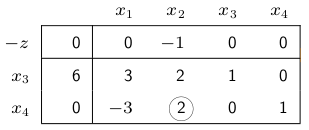
\includegraphics[width=0.5\textwidth]{images/cap6tab1.png}
  \caption{Il primo tableau}
  \label{cap6tab1}
\end{figure}

A questo punto vediamo che c'\`e un costo che \`e $\leq 0$, dunque
possiamo ancora migliorare la soluzione. Vediamo quale colonna dovremo
far uscire dalla base per far entrare la colonna $2$. Calcoliamo
dunque $\vartheta = \min\bigr\{\frac{6}{2}, \frac{0}{2} \bigr\} = 0$,
pertanto uscir\`a la colonna in relativa alla variabile
$x_4$. Effettuiamo dunque il pivoting dividendo l'ultima riga per
$2$. Alla riga $1$ invece sottriamo la nuova ultima riga moltiplicata
per due ed otteniamo il tableau in figura \ref{cap6tab2}.

\begin{figure}[h!]
  \centering
  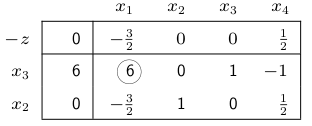
\includegraphics[width=0.5\textwidth]{images/cap6tab2.png}
  \caption{Il secondo tableau}
  \label{cap6tab2}
\end{figure}

Ancora una volta abbiamo una colonna con costo negativo, pertanto
operiamo ancora ed otteniamo il tableau in figura \ref{cap6tab3}.

\begin{figure}[h!]
  \centering
  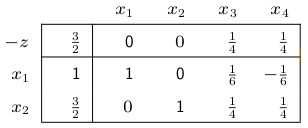
\includegraphics[width=0.5\textwidth]{images/cap6tab3.png}
  \caption{Il terzo tableau}
  \label{cap6tab3}
\end{figure}

A questo punto abbiamo ottenuto la soluzione ottima (dato che non ci
sono pi\`u colonne con costi negativi), tuttavia la soluzione presenta
valori frazionari. Dobbiamo dunque scegliere quale riga utilizzare
come generatrice. Prendiamo dunque in rassegna le varie righe e
vediamo quali tagli verrebbero fuori:

\begin{itemize}
\item {\bf riga 0} (frazionaria): $\frac{1}{4}x_3 + \frac{1}{4}x_4
  \geq \frac{1}{2}$ (dove $\frac{1}{2}$ \`e la parte frazionaria di
  $\frac{3}{2}$); da tale riga otteniamo $x_2 \leq 1$;

\item {\bf riga 1} (intera): $\frac{1}{6}x_3 + \frac{5}{6}x_4 \geq 0$
  (0 \`e la parte frazionaria di 1); qui otteniamo $x_1-x_2 \geq
  -\frac{1}{2}$;

\item {\bf riga 2} (frazionaria): $\frac{1}{4}x_3 + \frac{1}{4}x_4
  \geq \frac{1}{2}$. Ricaviamo, ovviamente, $x_2 \leq 1$.
\end{itemize}

Vediamo cosa succede scegliendo la riga 0. Dovremo aggiungere al
tableau la riga relativa a $-\frac{1}{4}x_3 - \frac{1}{4}x_4 + s_1 =
-\frac{1}{2}$ (Figura \ref{cap6tab4}).

\begin{figure}[h!]
  \centering
  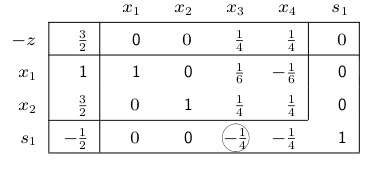
\includegraphics[width=0.5\textwidth]{images/cap6tab4.png}
  \caption{Quarto tableau}
  \label{cap6tab4}
\end{figure}

Dal momento che la riga relativa a $s_1$ \`e negativa dovremo far
uscire dalla base $s_1$. Quale facciamo entrare? Consideriamo gli
elementi negativi nella riga di $s_1$: a questo punto facciamo il
rapporto fra i costi di tale colonna e i suddetti elementi in valore
assoluto, vediamo qual \`e il minimo e quella sar\`a la colonna da far
entrare in base. 

\begin{figure}[h!]
  \centering
  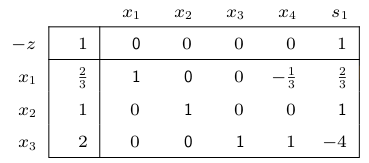
\includegraphics[width=0.5\textwidth]{images/cap6tab5.png}
  \caption{Quinto tableau}
  \label{cap6tab5}
\end{figure}

Abbiamo trovato una soluzione ottima, peccato che non sia intera
dunque dobbiamo pensare ai nuovi tagli. Scegliamo di apportare il
taglio relativo alla riga $1$ che \`e quella frazionaria. Il taglio
\`e $\frac{2}{3}x_4+ \frac{2}{3}s_1 \geq \frac{2}{3}$ che per
sostituzione ci d\`a $x_1 \geq x_2$. Moltiplicando per $-1$ ed
aggiungendo la variabile di slack, l'equazione di taglio \`e:
$-\frac{2}{3}x_4 - \frac{2}{3}s_1 + s_2 = - \frac{2}{3}$. Il tableau
assume ora la forma in figura \ref{cap6tab6}.

\begin{figure}[h!]
  \centering
  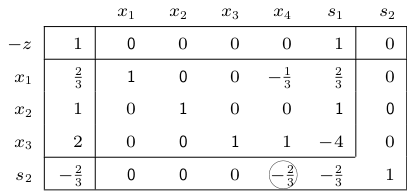
\includegraphics[width=0.5\textwidth]{images/cap6tab6.png}
  \caption{Sesto tableau}
  \label{cap6tab6}
\end{figure}

La soluzione non \`e ammissibile (per il primale) pertanto bisogna far
uscire $s_2$ dalla base. Ad entrare sar\`a $x_4$ perch\'e
$\frac{0}{|2/3|} < \frac{1}{|2/3|}$.

\begin{figure}[h!]
  \centering
  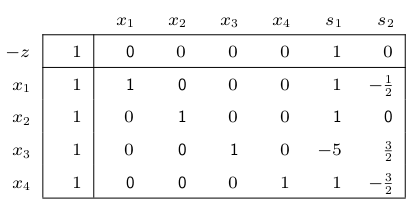
\includegraphics[width=0.5\textwidth]{images/cap6tab7.png}
  \caption{Settimo tableau}
  \label{cap6tab7}
\end{figure}

\begin{figure}[h!]
  \centering
  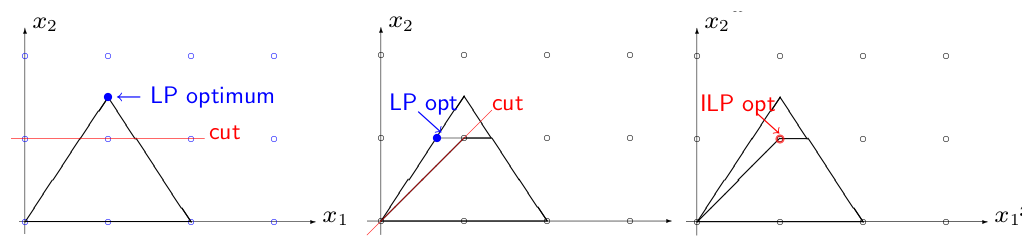
\includegraphics[width=\textwidth]{images/cap6esempio1.png}
  \caption{I tagli attuati}
  \label{cap6esempio1}
\end{figure}

Adesso finalmente la soluzione \`e ottima ed ammissibile per il
primale: $x_1 = x_2 = 1$, $z = -1$. In figura \ref{cap6esempio1} sono
visibili i tagli effettuati. $\blacktriangleleft$
\vspace{11pt}

\section{Branch and Bound}

Il {\bf branch and bound} \`e un metodo generale per la soluzione di
qualsiasi problema di natura combinatoria. Il metodo consiste, una
volta trovata una soluzione non intera, nello spezzare il problema in
due sottoproblemi disgiunti che considerino un arrotondamento ai due
interi pi\`u grande e pi\`u piccolo che racchiudono la variabile con
valore frazionario. Il metodo risulter\`a pi\`u chiaro con un esempio.

\vspace{11pt}
$\blacktriangleright$ {\bf Esempio}: sia dato il problema di ILP
seguente:

\vspace{11pt}
\begin{center}
\begin{tabular}{l}
$\min z^0 = c'x$ \\
$\phantom{mina}Ax= b$ \\
$\phantom{mina}x\geq 0, intero$ \\
\end{tabular}
\end{center}
\vspace{11pt}

Abbiamo chiamato il problema originale $P^0$; indicheremo anche i
sottoproblemi con la notazione $P^k, k = 0,1,2,\dots$, mentre
indicheremo con $z^k$ la soluzione del {\em k}-esimo problema.

Supponiamo che la soluzione del problema sia quella evidenziata in
figura \ref{cap6fig66}.

\begin{figure}[h!]
  \centering
  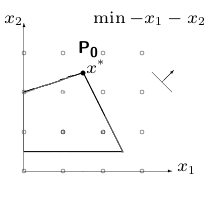
\includegraphics[width=0.4\textwidth]{images/cap6fig66.png}
  \caption{Soluzione al rilassamento continuo}
  \label{cap6fig66}
\end{figure}

Dal momento che la soluzione non \`e intera non possiamo fermarci ed
adotteremo il branch and bound. Vediamo di cosa consiste.

{\bf Branching}: la soluzione $x^0$ avr\`a almeno una componente
frazionaria (in questo caso guardando dal disegno vediamo che entrambe
son frazionarie, sia $x_1^0$, sia $x_2^0$). Consideriamo $x_1^0 =
\frac{3}{2}$. Tale valore \`e compreso fra 1 e 2, pertanto possiamo
generare due sottoproblemi aggiungendo al primo il vincolo $x_1 \leq
1$ ed al secondo $x_1 \geq 2$.
 
Possiamo dunque ricavare la regola: trovata una soluzione $z^k$ al
problema $P^k$ che abbia variabili frazionarie, possiamo prendere la
variabile frazionaria $x_i^k$ e suddividere il problema in due
sottoproblemi $P^{k+1}$ e $P^{k+2}$ corrispondenti con l'aggiunta dei
due vincoli $x_i \leq \lfloor x_i^k \rfloor$ e $x_i \geq \lfloor x_i^k
\rfloor + 1$. La soluzione ottima sar\`a la minima fra quelle trovate.

A questo punto torniamo all'esempio e vediamo come si procede. Una
volta aggiunti i vincoli indicati in precedenza abbiamo le due regioni
distinte che appaiono in figura \ref{cap6fig66bis}.

\begin{figure}[h!]
  \centering
  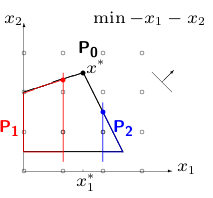
\includegraphics[width=0.4\textwidth]{images/cap6fig66bis.png}
  \caption{Branching}
  \label{cap6fig66bis}
\end{figure}
$\blacktriangleleft$
\vspace{11pt}

Ovviamente si pu\`o risolvere un problema per volta. Ci concentriamo
ad esempio su $P^2$ e troviamo la soluzione $x^2 = (2,\frac{3}{2})$ e
non essendo intera procediamo ad un'ulteriore ramificazione imponendo
$x_2 \leq \lfloor x_2^2 \rfloor = 1$ e $x_2 \geq \lfloor x_2^2 + 1
\rfloor = 2$. Il primo sottoproblema ottenuto ci d\`a ancora una
regione ammissibile, l'altro no, dunque \`e impossibile.

Il problema $P^4$ \`e risolto e risolvendo il problema $P^3$ troviamo
invece ancora una soluzione frazionaria quindi pu\`o essere ancora
ramificato.

Il procedimento che stiamo adottando per risolvere il problema pu\`o
essere rappresentato tramite l'{\bf albero decisionale binario}
(Figura \ref{cap6fig610}).

\begin{figure}[h!]
  \centering
  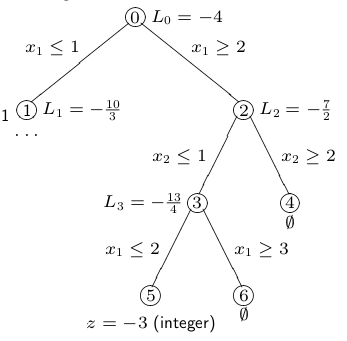
\includegraphics[width=0.6\textwidth]{images/cap6fig610.png}
  \caption{L'albero decisionale binario}
  \label{cap6fig610}
\end{figure}

Il problema principale costituisce {\bf nodo radice}. Ogni nodo \`e
congiunto da un {\bf ramo} ascendente al nodo che lo ha generato ({\bf
  progenitore}) e da esso partono due rami discendenti verso i due
figli (detti {\bf discendenti}) che pu\`o generare. I nodi privi di
figli son detti {\bf foglie}. Accanto ad ogni ramo viene indicata la
condizione che produce il nodo figlio mentre accanto ad ogni nodo
viene indicato il valore della soluzione del rilassamento continuo del
problema relativo.

{\bf Bounding}: se si continua a ramificare fino a quando nessun
nodo pu\`o pi\`u generare figli, allora la soluzione ottima del
problema originale $P^0$ \`e data dalla soluzione della foglia di
costo minimo.

Ritornando all'esempio, l'albero decisionale mostra che la soluzione
ottima del problema $P^2$ \`e $x=(2,1)$ di valore -3. Dovremmo a
questo punto generare i discendenti del nodo 1, tuttavia possiamo
risparmiarcelo (e risparmiarci molta fatica) grazie ai {\bf bound}
(limiti). Il valore della soluzione di $P^1$ \`e $L_1 =
-\frac{10}{3}$. Tale valore fornisce un {\bf lower bound} al valore
della soluzione ottima di $P^1$. Nessuna soluzione prodotta da $P^1$ o
dai suoi discendenti potr\`a avere un valore inferiore a $\lceil L_1
\rceil = -3$. Dato che abbiamo gi\`a trovato una soluzione che vale
$-3$ dall'altra parte dell'albero, sappiamo che l'esplorazione della
parte sinistra non potr\`a produrre una soluzione migliore, per cui la
soluzione trovata \`e gi\`a ottima e ci fermiamo.

In generale dunque: se {\em z} \`e il valore della miglior soluzione
intera trovata finora e per un problema $P^k$ si ha $\lceil L_k \rceil
\geq z$, allora non occorre risolvere il problema $P^k$ (si dice che
il corrispondente nodo viene {\bf ucciso}). Quando si deve risolvere
un problema di massimizzazione si parla invece di {\bf upper bound}
anzich\'e di {\em lower bound}. In ogni caso nell'albero decisionale
si preferisce rappresentare accanto ai noi il valore del bound gi\`a
arrotondato per eccesso o per difetto.

\section{Inserimento dei vincoli nel tableau}

Supponiamo di voler inserire nel tableau il vincolo $x_i \leq \lfloor
a \rfloor$, che in forma standard equivale a $x_i + s = \lfloor a
\rfloor$. Dato il tableau ottimo del simplesso, aggiungendo la riga
corrispondente si ottiene:

\begin{figure}[h!]
  \centering
  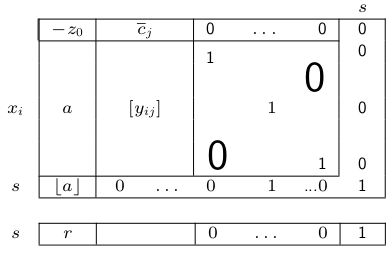
\includegraphics[width=0.6\textwidth]{images/cap6tab8.png}
  \caption{Inserimento dei vincoli nel tableau}
  \label{cap6tab8}
\end{figure}

A questo punto per\`o \`e necessario ottenere nuovamente
l'identit\`a. Per far ci\`o sottraiamo alla nuova riga, la riga di
$x_i$. Si ottiene dunque

\begin{figure}[h!]
  \centering
  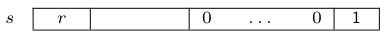
\includegraphics[width=0.6\textwidth]{images/cap6tab9.png}
  \caption{La nuova riga {\em s}}
  \label{cap6tab9}
\end{figure}

Avendo ottenuto nella prima colonna $r = \lfloor a \rfloor < 0$ \`e
necessario proseguire poi con l'algoritmo del simplesso.

Volendo al contrario imporre il vincolo $x_i \geq \lfloor a \rfloor +
1$, in forma standard $-x_i + s = - \lfloor a \rfloor -1 = t$, si
ottiene:

\begin{figure}[h!]
  \centering
  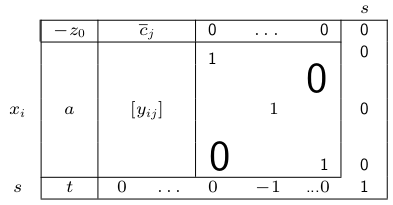
\includegraphics[width=0.6\textwidth]{images/cap6tab10.png}
  \caption{Inserimento del vincolo nel tableau}
  \label{cap6tab10}
\end{figure}

Tramite la somma della riga di $x_i$ alla riga $s$ otteniamo:

\begin{figure}[h!]
  \centering
  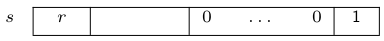
\includegraphics[width=0.6\textwidth]{images/cap6tab11.png}
  \caption{La nuova riga}
  \label{cap6tab11}
\end{figure}

Anche in questo caso dobbiamo proseguire con il metodo del simplesso
avendo ottenuto $r = a - \lfloor a \rfloor -1 < 0$.

\vspace{11pt}
$\blacktriangleright$ {\bf Esempio}: risolviamo tramite branch and
bound il seguente problema di ILP:

\vspace{11pt}
\begin{center}
  \begin{tabular}{l}
    $\max z = x_1 + 4x_2$\\
    $\phantom{min}x_1 + 3x_2 \leq 9$\\
    $\phantom{min}2x_1 - x_2 \geq 0$\\
    $\phantom{min}x_1, x_2 \geq 0$, interi\\
  \end{tabular}
\end{center}
\vspace{11pt}

Essendo 0 il termine noto del secondo vincolo, possiamo moltiplicare
per -1. Non lo potremmo fare in caso contrario perch\'e non posiamo
modificare il segno dei termini noti dato che compaiono nella prima
colonna del tableau. 

Il modello in forma standard \`e:

\vspace{11pt}
\begin{center}
  \begin{tabular}{l}
    $\min -z = -x_1 - 4x_2$\\
    $\phantom{min}x_1 + 3x_2 + x_3 = 9$\\
    $\phantom{min}-2x_1 + x_2 + x_4 = 0$\\
    $\phantom{min}x_1, x_2, x_3, x_4 \geq 0$, interi\\
  \end{tabular}
\end{center}
\vspace{11pt}

Con l'algoritmo del simplesso otteniamo il tableau:

\begin{figure}[h!]
  \centering
  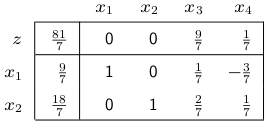
\includegraphics[width=0.55\textwidth]{images/cap6tab12.png}
  \caption{Il tableau ottenuto}
  \label{cap6tab12}
\end{figure}

La soluzione non \`e intera pertanto dovremo procedere con il branch
and bound. La soluzione ci d\`a un {\bf lower bound} pari a $L =
\lceil -\frac{81}{7} \rceil = -11$.

Per ramificare scegliamo la variabile $x_1$ ed imponiamo la condizione
$x_1 \leq 1$ che in forma standard si traduce in $x_1 + x_5 =
1$. Inserendo tale regola nel tableau ed effettuando la sottrazione
con la riga 1 otteniamo il tableau sul quale eseguire l'algoritmo del
simplesso duale (eseguiamo tale algoritmo perch\'e vi \`e un valore
negativo nella prima colonna). Lo vediamo in alto in figura
\ref{cap6tab13}. Il secondo tableau \`e quello che otteniamo con il
simplesso duale e ci porta alla soluzione intera $-9$. Tale soluzione
\`e maggiore del lower bound, pertanto non \`e ottima per
l'ILP.

\begin{figure}[h!]
  \centering
  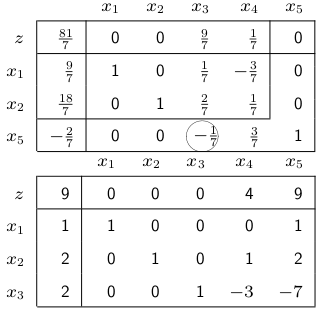
\includegraphics[width=0.55\textwidth]{images/cap6tab13.png}
  \caption{Il tableau su cui operare con il simplesso duale}
  \label{cap6tab13}
\end{figure}

Ramifichiamo perci\`o anche dall'altro lato usando la condizione $x_1
\geq 2$ (che in forma standard \`e $-x_1 + x_6 = -2$) e, una volta
inserita tale condizione nel tableau, le sommiamo riga 1.

\begin{figure}[h!]
  \centering
  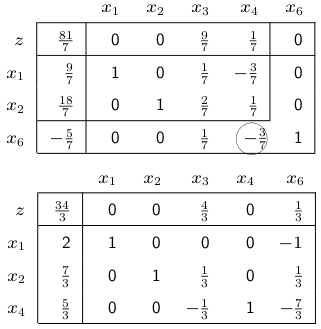
\includegraphics[width=0.55\textwidth]{images/cap6tab14.png}
  \caption{Il secondo ramo}
  \label{cap6tab14}
\end{figure}

La soluzione non \`e intera e d\`a un lower bound pari a $\lceil
-\frac{34}{3} = -11$.

A questo punto l'albero \`e costituito dai nodi 0, 1 e 2 come si pu\`o
vedere in figura \ref{cap6albero}.

\begin{figure}[h!]
  \centering
  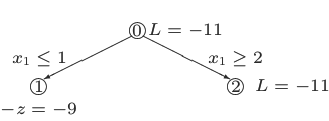
\includegraphics[width=0.7\textwidth]{images/cap6albero.png}
  \caption{Albero decisionale}
  \label{cap6albero}
\end{figure}

Dal momento che il lower bound del problema 2 \`e migliore della
soluzione \underline{intera} trovata sul ramo 1 si pu\`o continuare a
ramificare il ramo 2. Scegliendo la variabile $x_2$ ed imponendo per
prima la condizione $x_2 \leq 2$ si ottiene il tableau in alto in
figura \ref{cap6tab15}. 

\begin{figure}[h!]
  \centering
  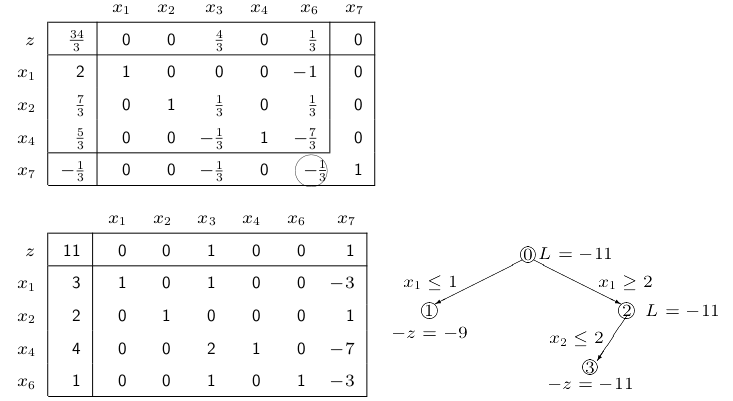
\includegraphics[width=\textwidth]{images/cap6tab15.png}
  \caption{Nuovo tableau}
  \label{cap6tab15}
\end{figure}

Procedendo con il simplesso duale arriviamo al secondo tableau ed alla
soluzione intera di valore $-11$ pari al lower bound del nodo padre,
dunque non si deve esplorare il secondo figlio del nodo 2 e si \`e
trovata la soluzione ottima del problema: $x_1 = 3$, $x_2 =
2$. $\blacktriangleleft$
\vspace{11pt}

\section{Strategie di esplorazione}

La sequenza di esplorazione dei nodi influisce sulla velocit\`a di
convergenza dell'algoritmo branch-and-bound, pertanto fondamentale \`e
la decisione riguardo alla sequenza in cui generare ed esplorare i
nodi dell'albero decisionale.

\subsection{Depth-first}

Questo metodo di ricerca opera in profondit\`a ed opera come segue: si
calcola $L(P^0)$, si genera il primo figlio $P^1$ e se ne calcola il
lower bound. Si genera il primo figlio di $P^1$ e cos\`i via. In
generale ({\bf forward step}) si genera un figlio dell'ultimo nodo
$P^k$ generato finch\'e:

\begin{itemize}
\item si ottiene un problema facilmente risolubile ed eventualmente
  si aggiorna {\em z}
\item $L(P^k)\geq z$
\item $P^k$ non ha figli ammissibili non ancora esplorati.
\end{itemize}

In questi casi si effettua il {\bf backtracking}, cio\`e si risale al
padre di $P^k$ (chiamiamolo $P^p$) e se $L(P^p)<z$ si genera il suo
figlio successivo quindi il primo figlio di questo, e cos\`i via. In
caso contrario si risale al padre di $P^p$. Si termina quando si cerca
di risalire al di sopra di $P^0$.

{\bf Vantaggi:} mantiene un basso numero di nodi attivi e produce una
struttura in cui ogni nodo \`e padre o figlio del nodo precedentemente
trattato. Richiede dunque strutture semplici per la memorizzazione
dell'albero decisionale e porta ad una relativa facilit\`a di
implementazione dell'algoritmo. La strategia tende inoltre a produrre
rapidamente soluzioni ammissibili, aumentando la possibilit\`a di
uccidere nodi.

\subsection{Lowest-first}

Privilegia i nodi con pi\`u basso lower-bound. Si calcola $L(P^0)$ e
si definisce $\prod := \{ P^0 \}$ (insieme dei nodi attivi). Ad ogni
iterazione si rimuove da $\prod$ il nodo con pi\`u basso lower bound e
si generano tutti i suoi figli. Si calcolano dunque i relativi lower
bound. Se ci sono nodi facilmente risolubili eventualmente si aggiorna
{\em z}. Si inseriscono in $\prod$ i nodi $P^k$ non risolubili e tali
che $L(P^k)<z$. Si termina quando $\prod$ \`e vuoto o contiene solo
nodi tali che $L(P^k)\geq z$. Per problemi di massimizzazione si parla
di {\bf highest-first}.

{\bf Vantaggi:} esplora per primo sempre il nodo pi\`u promettente (ma
richiede un tempo di calcolo elevato) e quindi trova la soluzione
ottima esplorando un numero relativamente basso di nodi.

{\bf Svantaggi:} mantiene un alto numero di nodi attivi senza nessuna
relazione tra nodo attuale e nodo precedente; richiede dunque
strutture dati pi\`u complesse e l'implementazione \`e pi\`u
faticosa. Le soluzioni non vengono prodotte rapidamente.

\subsection{Depth-first rivisitato}

Unisce i vantaggi delle due strategie precedenti, ma nel forward step
si generano tutti i figli del nodo attuale, si calcolano i loro lower
bound e si prosegue l'esplorazione dal figlio con minimo lower bound e
nel backtracking si riprende l'esplorazione dal nodo non esplorato con
minimo lower bound fra i figli del nodo cui si \`e risaliti.

Vi \`e un aggravio computazionale, ma \`e compensato dall'avere una
ricerca pi\`u efficiente.

\subsection{Breadth-first}

Questa modalit\`a \`e usata pi\`u di rado. Si generano tutti i figli
di $P^0$ e di ogni figlio di $P^0$ non facilmente risolubile si
generano tutti i figli e cos\`i via.

Questa strategia, che pu\`o anche prevedere il calcolo di bound, viene
usata, ad esempio, quando interessano tutte le soluzioni ammissibili
del problema o tutte quelle con un certo valore massimo. 

\section{Altri problemi di ottimizzazione}

Il problema lineare pi\`u generale \` la {\bf programmazione lineare
  intera mista} ({\bf MILP}, {\em Mixed Integer Linear Programming}).

\vspace{11pt}
\begin{center}
  \begin{tabular}{l}
    $\min c'x$\\
    $\phantom{min}Ax = b$\\
    $\phantom{min}x_j \geq 0,\phantom{aaaaaaaaaa}j \in N$\\
    $\phantom{min}x_j \geq 0 $ e intero, $\phantom{aaa}j \in \bar{N}$\\
  \end{tabular}
\end{center}
\vspace{11pt}

\`E una generalizzazione sia dei problemi di LP (che sono il caso
particolare in cui $\bar{N} = \emptyset$) dei problemi di ILP (che
sono il caso particolare in cui $N = \emptyset$). Questa tipologia di
problemi si risolve con le metodologie viste per i problemi di
programmazione lineare intera, considerando per il branching soltanto
le variabili dell'insieme $\bar{N}$ che risultino frazionarie.

Un'altra tipologia di problemi \`e rappresentata invece dalla {\bf
  programmazione lineare binaria} o $0-1$ ({\bf LP01}), nella quale le
variabili possono assumere soltanto valori binari:

\vspace{11pt}
\begin{center}
  \begin{tabular}{l}
    $\min c'x$\\
    $\phantom{min}Ax = b$\\
    $\phantom{min}x_j \in \{ 0, 1\} \forall j$\\
  \end{tabular}
\end{center}
\vspace{11pt}

Questa tipologia di problemi viene solitamente espressa come problema
di massimizzazione nella forma:

\vspace{11pt}
\begin{center}
  \begin{tabular}{l}
    $\max \sum\limits_{j=1}^{n} p_jx_j$\\
    $\phantom{min}\sum\limits_{j=1}^n w_jx_j \leq c$\\
    $\phantom{min}x_j \in \{ 0, 1\} (j =1, \dots, n)$\\
  \end{tabular}
\end{center}
\vspace{11pt}

ed \`e noto come {\bf problema knapsack 0-1} ({\em KP01}). Questo nome
\`e dovuto alla seguente interpretazione: un autostoppista vuole
riempire il proprio zaino ({\em knapsack}) scegliendo fra {\em n}
oggetti: ogni oggetto {\em j} ha un valore ({\em profitto}) $p_j$ ed
un peso $w_j$. Lo zaino ha capacit\`a {\em c}. L'autostoppista vuole
dunque scegliere un sottoinsieme di oggetti di peso complessivo non
superiore a $c$ che abbia massimo profitto complessivo. Noi assumeremo
che $w_j \leq c \forall j$ e $\sum\limits_{j=1}^n w_j > c$, nonch\'e
che $p_j$, $w_j$ e {\em c} siano interi positivi.

\section{Problema Knapsack 0-1}

Vediamo in dettaglio il problema knapsack binario. Ordiniamo per
comodit\`a gli elementi secondo valori non crescenti del profitto per
unit\`a di peso (dal pi\`u promettente al meno promettente), dunque
assumeremo:

\begin{center}
$\frac{p_1}{w_1} \geq \frac{p_2}{w_2} \geq \dots \geq \frac{p_n}{w_n}$  
\end{center}

Adotteremo un albero binario in cui al livello {\em k} ({\em
  k=1,\dots,n}) decideremo se porre o meno in soluzione l'oggetto {\em
  k}. La strategia che prenderemo in considerazione sar\`a la {\em
  depth-first}. Al primo passo si generano i due nodi $x_1 = 1$ ed
$x_1 = 0$ e ad ogni iterazione, se esiste nodo attivo generato da
$x_j=1$, si ramifica da questo, altrimenti si ramifica dall'ultimo
nodo attivo generato da $x_j = 0$. In questo modo l'insieme dei nodi
attivi contiene sempre al pi\`u un nodo generato da una condizione
$x_j = 1$ e uno o pi\`u nodi generati da $x_j = 0$.

In merito all'{\bf upper bound} (\`e {\em upper} e non {\em lower}
essendo un problema di massimo), il rilassamento continuo di un
problema binario viene calcolato sostituendo $x_j \in \{0,1\}$ con $j
= 1, \dots, n$, $0 \leq x_j \leq 1$. In questo caso il calcolo non
richiede l'algoritmo del simplesso e pu\`o essere fatto come segue.
Ricordando che abbiamo posto gil oggetti in maniera ordinata, possiamo
calcolare l'upper bound {\em U} usano la capacit\`a nel miglior modo
possibile:

\begin{quote}
si inseriscono uno dopo l'altro gli elementi migliori, frazionando il
primo che non pu\`o essere inserito interamente.  
\end{quote}

Possiamo considerare delle frazioni in quanto stiamo risolvendo il
rilassamento lineare.

\begin{quote}
Formalmente:
\begin{center}
$s := \min \{i: \sum\limits_{j=1}^{i}w_j > c \}$ (elemento critico);
  $\bar{c} := c-\sum\limits_{j=1}^{s-1}w_j$;\\
$U := \biggr\lfloor \sum\limits_{j=1}^{s-1}p_j + \bar{c}\frac{p_s}{w_s}\biggr\rfloor$
\end{center}
\end{quote}
  
Una conseguenza importante \`e che l'upper bound di un nodo generato
da $x_j = 1$ \`e pari all'upper bound del nodo padre. \`E inoltre
interessante notare che per ogni nodo l'upper bound del figlio di
sinistra non \`e peggiore di quello del figlio di destra, per cui si
segue implicitamente una strategia {\em depth-first rivisitata}.

\vspace{11pt}
$\blacktriangleright$ {\bf Esempio}: sia dato un problema $KP01$ con
$n=5$, $p' = (12,12,7,6,2)$, $w'=(4,5,3,3,2)$ e $c=10$ (gli elementi
sono gi\`a ordinati).

In figura \ref{cap6fig613} \`e possibile osservare l'albero generato
dal branch and bound. Gli upper bound sono sottolineati se sono stati
calcolati, altrimenti vuol dire che sono stati ricavati dal bound del
padre. Il numero del nodo indica l'ordine di esplorazione.

\begin{figure}[h!]
  \centering
  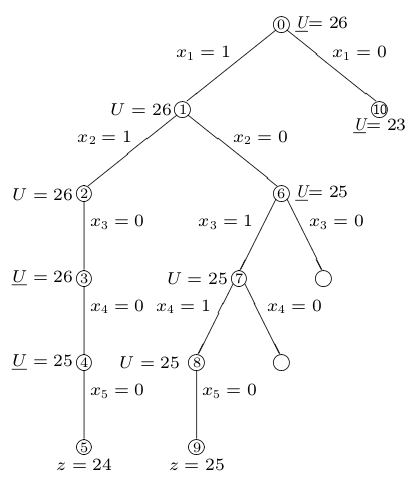
\includegraphics[width=0.65\textwidth]{images/cap6fig613.png}
  \caption{Albero decisionale}
  \label{cap6fig613}
\end{figure}

L'upper bound iniziale \`e $U = \lfloor 12+12+\frac{7}{3} \rfloor =
26$. Dopo aver generato i nodi 1 e 2 con lo stesso upper bound, la
capacit\`a residua non \`e sufficiente per considerare altri elementi
perch\'e $10 - (1\cdot w_1 + 1\cdot w_2) = 1$ ed il costo degli altri
elementi \`e $> 1$. Si trova dunque la soluzione $x'=(1,1,0,0,0)$ di
valore $z=24$ (cio\`e $1\cdot p_1 + 1\cdot p_2$).

Si effettuano perci\`o quattro backtracking fino a trovare il nodo 1,
da cui si ramifica. Calcoliamo l'upper buond del nodo 6 e riprendiamo
la discesa depth-first trovando la soluzione $x' = (1,0,1,1,0)$ di
valore $z=25$. Non si deve pertanto ramificare i rami 7 e 6 perch\'e
avrebbero $U \leq z$. Si ramifica quindi dal nodo 0 e si calcola
l'upper bound del nodo 10, $U = 23 < z$. Non essendoci altri nodi
attivi termina l'esecuzione con la soluzione ottima trovata prima
$x'=(1,0,1,1,0)$ di valore 25. $\blacktriangleleft$
\vspace{11pt}

L'algoritmo pu\`o essere implementato in maniera semplice. Basta
mantenere un puntatore {\em k} al livello corrente ed il vettore delle
decisioni. Ad esempio al quarto livello potremmo avere $k=4$ e
$x'=(1,0,1,1,-,-)$. Gli elementi $x_1,\dots,x_k$ hanno i valori
attualmente fissati nell'albero e $x_{k+1},\dots,x_n$ sono indefiniti.

Il passo principale dell'algoritmo \`e il seguente:

\vspace{11pt}
\begin{center}
\begin{tabular}{||l||}
\hline\hline
\# forward step\\
$k:=k+1;$\\
{\bf if} $w_k \leq c - \sum\limits_{j=1}^{k-1}w_jx_j$ {\bf then}
$x_k:=1$\\
{\bf else}\\
\phantom{aa}{\bf begin}\\
\phantom{aaaa}$x_k := 0;$\\
\\
\phantom{aaaa}$U :=\phantom{a}$ upper bound per il nodo attuale;\\
\phantom{aaaa}{\bf while} $U \leq z$ (= miglior soluzione trovata) {\bf do}\\
\phantom{aaaaaa}{\bf begin}\\
\\
\phantom{aaaaaaaa}\# backtraking\\
\phantom{aaaaaaaa}$k := \max\{ j<k: x_j = 1\};$\\
\phantom{aaaaaaaa}$x_k:=0$;\\
\phantom{aaaaaaaa}$U :=\phantom{a}$ upper bound per il nodo attuale\\
\phantom{aaaaaa}{\bf end}\\
\phantom{aaaa}{\bf end}\\
\hline\hline
\end{tabular}
\end{center}
\vspace{11pt}

\section{Algoritmi branch and cut}

Un approccio oggi fortemente usato consiste nella combinazione fra i
metodi {\em branch and bound} e {\em cutting planes} e va sotto il
nome di {\bf branch-and-cut}. Un algoritmo di questo tipo ha una
struttura branch and bound, ma:

\begin{quote}
ad ogni nodo dell'albero decisionale con soluzione non intera si
generano tagli, cercando di trovare una soluzione intera, o almeno di
ottenere un bound migliore.
\end{quote}

Non si usano di solito tagli di Gomory in quanto dipendono dalle
condizioni imposte ai nodi progenitori per cui occorrerebbe
memorizzare i tagli relativi a ciascun nodo. Si usano invece dei tagli
particolari detti {\bf global cuts}, validi per tutto l'albero
decisionale e memorizzati in una struttura dati apposita ({\bf pool}
dei vincoli). Le operazioni eseguite ad ogni nodo dell'albero
decisionale possono essere espresse come:

\small
\vspace{11pt}
\begin{center}
\begin{tabular}{||l||}
\hline\hline
{\bf while} $x^*$ non \`e intera {\bf and} non \`e stato raggiunto un
limite di iterazioni {\bf do}\\
\phantom{aa}{\bf if} il pool contiene tagli violati da $x^*$ {\bf then}\\
\phantom{aaaa}{\bf begin}\\
\phantom{aaaaaa}scegli uno o pi\`u tagli non ancora utilizzati;\\
\phantom{aaaaaa}aggiungi i tagli al problema corrente;\\
\phantom{aaaaaa}$x^* :=\phantom{a}$ soluzione del rilassamento continuo\\
\phantom{aaaa}{\bf end}\\
\phantom{aa}{\bf else} genera nuovi tagli e aggiungili al pool
{\bf end}\\
\hline\hline
\end{tabular}
\end{center}
\vspace{11pt}
\normalsize

La principale difficolt\`a per la realizzazione di questi algoritmi
\`e nella ricerca di metodi in grado di produrre dei tagli
efficienti. Esistono anche implementazioni pi\`u complesse che
prevedono di calcolare anche dei tagli locali {\em local cuts}, validi
solo per i discendenti di determinati nodi dell'albero decisionale.

\section{Software per LP, ILP e MILP}

Per problemi di grosse dimensioni servono software specializzati che
sappiano risolvere le seguenti problematiche:

\begin{itemize}
\item {\bf Stabilit\`a numerica}: poich\`e le operazioni sono in
  floating point, si generano errori di arrotondamento che tendono a
  propagarsi e causare istabilit\`a. Un esempio \`e dato dalla
  divisione di 1 per 3 che da $0.3e\bar{3}$. Moltiplicando per 3, il
  risultato \`e $0.99\bar{9}$. Se lo sottraiamo a 1 otteniamo
  $0.00\dots 01$ e sar\`a necessario decidere se ci\`o corrisponde ad
  un valore diverso da 0 e quindi potr\`a essere usato come pivot o
  meno.
  
\item {\bf Velocit\`a di esecuzione}: se un problema in forma standard
  ha centinaia di migliaia di variabili e vincoli , eseguire ad ogni
  iterazione le operazioni su un tableau sarebbe proibitivo. I
  software utilizzano una versione rivista dell'algoritmo del
  simplesso ({\bf Revised Simplex Algorithm}) che gestisce solo
  l'inversa della matrice base, dalla quale si possono calcolare tutte
  le informazioni richieste dall'algoritmo.

\item {\bf Sparsit\`a della matrice}: nei problemi industriali di
  grandi dimensioni la matrice {\em A} contiene molte celle pari a 0
  per cui sono necessarie tecniche particolari per gestire
  efficientemente l'inversa della matrice base.
\end{itemize}

I principali sistemi software commerciali per la programmazione lineare, intera e
mista sono:

\begin{itemize}
\item CPLEX Optimizer (IBM);
\item Gurobi Optimizer (Gurobi Optimization);
\item LINDO e LINGO solvers (LINDO Systems);
\item XPRESS-Optimizer (FICO);
\item MPL modeling system (Maximal Software).
\end{itemize}

Nel campo open source troviamo invece:

\begin{itemize}
\item Clp;
\item lpsolve;
\item SCPI.
\end{itemize}

\end{document}

